%----------------------------------------------------------------------------------------
%	SECTION 4.3
%----------------------------------------------------------------------------------------

\section{The Mean Value Theorem.}

\begin{lemma}[Rolle's Theorem]\label{4.3.1}
    Let $a,b \in \R$, with  $a \neq b$. If  $f$ is continous on  $[a,b]$, and differentiable on 
    $(a,b)$, and if  $f(a)=f(b)$, then there is a  $c \in (a,b)$ such that $f'(c)=0$.
\end{lemma}
\begin{proof}
    By the extreme value theorem,  $f$ is continous, so  $f$ has a finite maximum  $M$ and 
    a finite minimum  $m$ on  $[a,b]$. If  $M=m$, then  $f$ is a constant finction and 
    $f'(c)=0$ for all  $c \in (a,b)$. Now suppose that $M \neq m$. Since $f(a)=f(b)$, then there 
    must be some  $c \in (a,b)$ such that $f(c)=M$ or  $f(c)=m$. Without loss of generality, if \
    $f(c)=M$, then we have that $f(x) \leq f(c)$ for all  $x \in [a,b]$, then 
    $f(c)-f(x) \geq 0$, so $ \frac{f(c)-f(x)}{c-x} \geq 0$, on the other hand we have 
    $f(x)-f(c) \leq 0$, and  $\frac{f(x)-f(c)}{x-c} \leq 0$; taking limits as $x \rightarrow c$, we 
    then get that  $0 \leq f'(c) \leq 0$. Therefore  $f'(c)=0$. A similar argument follows 
    for  $f(c)=m$.
\end{proof}

\begin{remark} 
    The continuity hypothesis in Rolle's theorem cannot be relaxed, neither can the 
    assumption that $f(a)=f(b)$, and  $f$ being differentiable on  $(a,b)$.
\end{remark}

\begin{example}
    Consider the function $f(x)=x$ for  $x \in [0,1)$, and $f(x)=0$ everywhere else. 
    Rolle's theorem fails cause $f$ is not continous at  $x=1$. Likewise,  $f=|x|$ is 
    not differentiable at  $x=0$, and so Rolle's theorem failes for that as well.
\end{example} 

\begin{theorem}[The Mean Value Theorem]\label{4.3.2}
    Suppose that $a,b \in \R$, with  $a<b$. Then:
        \begin{enumerate}[label=(\arabic*)]
            \item If $f, g$ are continuous on  $[a,b]$, and differentiable on  $(a,b)$, then 
                there is a $c \in (a,b)$ such that $f'(c)(g(b)-g(a))=g'(c)(f(b)-f(a))$.

            \item If $f$ is continuous on  $[a,b]$, and differentiable on  $(a,b)$, then there is 
                a  $c \in (a,b)$ such that $f'(c)(b-a)=f(b)-f(a)$.
        \end{enumerate}
\end{theorem}
\begin{proof}
    We need only prove $(1)$. Let  $h(x)=f(x)(g(b)-g(a))-g(x)(f(b)-f(a))$. We have that 
    $h$ is continous on  $[a,b]$, differentiable on $(a,b)$, and we also see that $h(a)=h(a)$.
    Then by Rolle's theorem, there is some  $c \in (a,b)$ for which $h'(c)=0$. Thus 
    we have that  $0=f'(c)(g(b)-g(a))-g'(c)(f(b)-f(a))$. We are done. To prove $(2)$ 
    we take  $g$ to the identity function.
\end{proof}

\begin{figure} 
    \centering
    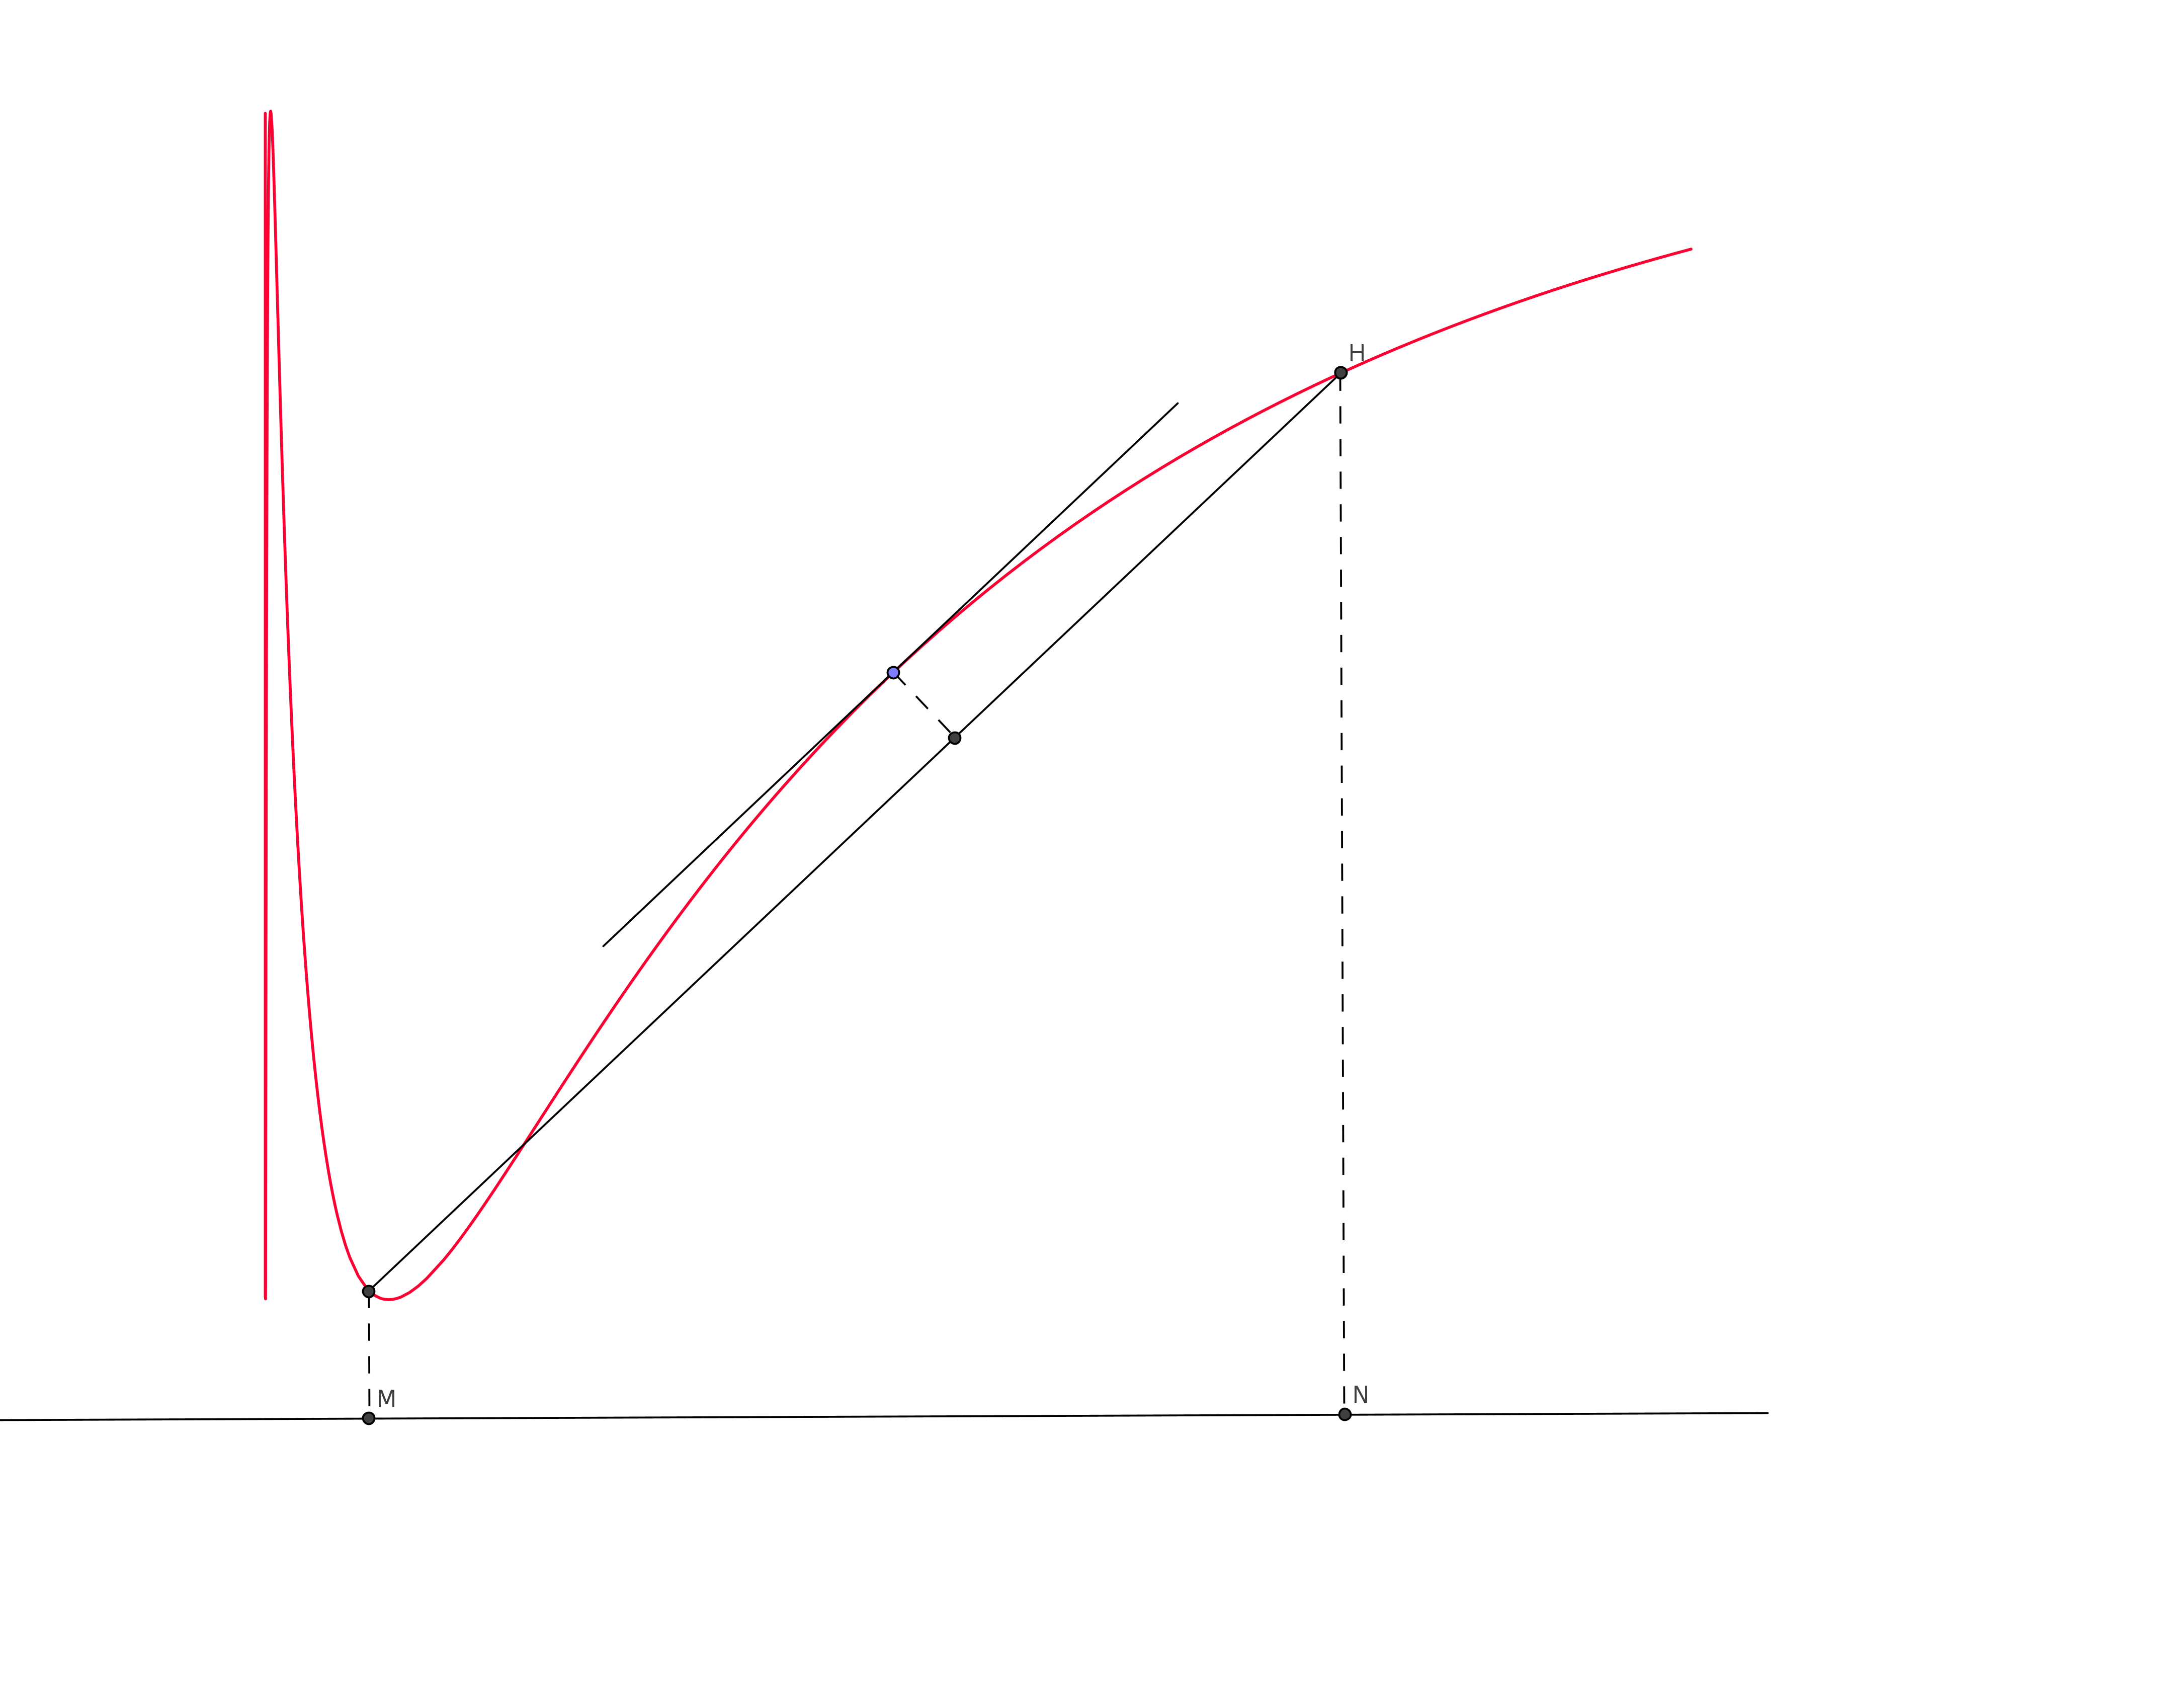
\includegraphics[scale = 0.3]{figures/meanValueTheorem.png}
    \caption{The Mean Value Theorem}
    \label{fig4.1}
\end{figure}

\begin{example}
    Show that $e^x \geq 1+x$.		
\end{example}
\begin{solution}
    Notice that for $f(x)=e^x$,  $f'(x)=e^x$. We also have that  $e^x>1$ when  $x>0$, 
    and $e^x<1$ when  $x<0$. Then consider the intervals  $(x,0)$ and $(0,x)$. By the 
    mean value theorem, there is a  $c \in (0,x)$ for which $e^x-1=xe^c$. Since $e^c>1$, then 
    we get that  $e^x-1 \geq x$. We get the same result for  $(x,0)$.
\end{solution}

\begin{theorem}[Bernoulli's Inequallity]\label{4.3.3}
   Let $\alpha>0 \in \R$ and let  $\delta \geq -1$. If  $0<\alpha \leq 1$, then 
   $(1+\delta)^{\alpha} \heq 1+\alpha\delta$, and if  $\alpha >1$ then $(1+\delta)^{\alpha} \heq 1+\alpha\delta$
\end{theorem}

\begin{theorem}[L'Hospital's Rule]\label{4.3.4}
    Let $a$ be an extended real number, and let  $I$ be an open interval containing  $a$
    in it's interior, or as an endpoint. Suppose that  $f$ and  $g$ are differentiable on  
    $I \blackslash \{a\}$, and that  $g(x), g'(x) \neq 0$ for all  $x \in I \blackslash \{a\}$. 
    Suppose further that  $A=\lim{f}=\lim{g}$ as  $a \rightarrow a$, for  $x \in I$ is either $0$ 
    or  $\infty$. If  $B=\lim{\frac{f}{g}}$ as $x \rightarrow a$ exists as an extended real number
    then:
        \begin{equation}
            \lim_{x \rightarrow a}{\frac{f}{g}}=\lim_{x \rightarrow a}{\frac{f'}{g'}}		
        \end{equation} 
\end{theorem}
\begin{proof}
    Let $\{x_n\} \subseteq I$, such that  $x_n \rightarrow a$ as  $n \rightarrow \infty$. Then by the sequential 
    characterization, it suffices to show that  $ \frac{f(x_n)}{g(x_n)} \rightarrow B$ as 
    $n \rightarrow \infty$. Assume that $B \in \R$. By the mean value theorem, we have 
    that  $g(x)-g(y) \neq 0$.

    Now suppose that  $A=0$, and  $a \in \R$. Extending  $f$ and  $g$ to  $I \cup \{a\}$ by 
    $f(a)=g(a)=0$, then  $f$ and  $g$ are continuous ove  $I \cup \{a\}$, and differentiable 
    over  $I \backslash \{a\}$. Then there is a $c_n$ between  $x_n$ and  $a$ such that 
        \begin{equation*}
            \frac{(x_n)-f(a)}{g(x_n)-g(a)}=\frac{f'(c_n)}{g'(g(c_n)}
        \end{equation*}
    We also have that $\lim{c_n}=\lim{x_n}=a$ as  $n \rightarrow \infty$ by the squeeze theorem.  
    Then 
        \begin{equation*}
            \lim_{n \rightarrow \infty}\frac{f(x_n)}{g(x_n)}=\lim_{x \rightarrow \infty}\frac{f'(c_n)}{g'(c_n)}=B
        \end{equation*}

    Now suppose without loss of generality that $A=\infty$, and that  $a \in \R$.Since $x_n \rightarrow a$, 
    for each $n,k \in \N$, by the mean value theorem, we there is a  $c_{k,n}$ between  
    $x_k$ and $x_n$, such that:
        \begin{equation*}
            \frac{f(x_n)}{g(x_n)}=\frac{f(x_k)}{g(x_n)}-\frac{f(x_n)-f(x_k)}{g(x_n)}
        \end{equation*}
    Then we get:
        \begin{equation*}
            \frac{f(x_n)}{g(x_n)}=\frac{f(x_k)}{g(x_n)}-\frac{1}{g(x_n)}
                                (\frac{(g(x_n)-g(x_k))f'(c_{k,n})}{g'(c_{k,n})})
        \end{equation*}
    simplifying and distributing the appropriate terms we get
        \begin{equation*}
            \frac{f(x_n)}{g(x_n)}=\frac{f(x_k)}{g(x_n)}-\frac{g(x_k)f'(c_{k,n})}{g(x_n)g'(c_{k,n})}
            +\frac{f'(c_{k,n})}{g'(c_{k,n})}
        \end{equation*} 
    Taking limits, we then get:
        \begin{equation*}
            \lim_{k,n \rightarrow \infty}{\frac{f(x_n)}{g(x_n)}}=
            \lim_{k,n \rightarrow \infty}{\frac{f'(c_{k,n})}{g'(c_{k,n})}}=B
        \end{equation*}
    
    Now suppose without loss of generality that $a = \infty$. Then choose $c$ such that 
    $(c,\infty) \subseteq I$. Then for each  $y \in (0,\frac{1}{c})$, let $\phi(y)=f(\frac{1}{y})$. 
    and $\psi(y)=g(\frac{1}{y})$. 
        \begin{equation*}
            \frac{\phi'(y)}{\psi'(y)}=\frac{f'(\frac{1}{y})}{g'(\frac{1}{y})}
        \end{equation*}
    so let $x=\frac{1}{y}$, since $\phi$ and  $\psi$ satisfy the above cases, we are done i.e.
        \begin{equation*}
            \lim_{x \rightarrow \infty}{\frac{f(x)}{g(x)}}=
            \lim_{y \rightarrow 0}{\frac{\phi(y)}{\psi(y)}}=
            \lim_{y \rightarrow 0}{\frac{\phi'(y)}{\psi'(y)}}=
            \lim_{x \rightarrow \infty}{\frac{f'(x)}{g'(x)}}
        \end{equation*} 
\end{proof}
